\documentclass[conference]{IEEEtran}

\ifCLASSINFOpdf

\else

\fi

% correct bad hyphenation here
\hyphenation{op-tical net-works semi-conduc-tor}

\usepackage{graphicx}
\usepackage{todonotes}
\usepackage{booktabs}


\begin{document}

%
% paper title
% Titles are generally capitalized except for words such as a, an, and, as,
% at, but, by, for, in, nor, of, on, or, the, to and up, which are usually
% not capitalized unless they are the first or last word of the title.
% Linebreaks \\ can be used within to get better formatting as desired.
% Do not put math or special symbols in the title.
\title{Architekturdokumentation\\Mensch \"argere Dich nicht!}


% author names and affiliations
% use a multiple column layout for up to three different
% affiliations
\author{\IEEEauthorblockN{Martin Puse}
\IEEEauthorblockA{
853001}
\and
\IEEEauthorblockN{Marcel Pillich}
\IEEEauthorblockA{863121}
}

% make the title area
\maketitle

% As a general rule, do not put math, special symbols or citations
% in the abstract
\begin{abstract}
Die vorliegende Arbeit enth\"alt eine detaillierte Beschreibung einer Java-Applikation f\"ur des Spiels "Mensch \"argere Dich nicht",
welche f\"ur Spieleprogrammierer und Spieledesigner gleicherma\ss en geeignet ist. Ziel war es, dass der Programmierer
sich um Erscheinungsbild und Regeln des Spiels k\"ummern kann, ohne selber Spielfelder designen zu m\"ussen, wohingegen der Designer keine
Programmierkenntnisse ben\"otigt, um neue Spielfelder hinzuzuf\"ugen und zu testen. Zu diesem Zweck wurden eine Grammatik f\"ur die Spielfelder
und ein Generator, welcher die Grammatiken verarbeitet und automatisiert Code erzeugt, erstellt. Die dahinterliegende Idee, die Spielfelder
nicht auf Positions-, sondern Knoteninformationen zu basieren, wird ausf\"uhrlich dargestellt.
Schlussendlich werden Weiterentwicklungsm\"oglichkeiten des Prototyps pr\"asentiert.
\end{abstract}

\IEEEpeerreviewmaketitle



\section{Einleitung}
% no \IEEEPARstart
"Mensch \"argere Dich nicht" ist ein Brettspiel f\"ur bis zu 4 Personen. Es z\"ahlt zu den Klassikern im deutschsprachigen Raum und wurde 1907/1908 von Josef Friedrich Schmidt in Anlehnung an das englische Spiel Ludo erfunden, die Urspr\"unge finden sich jedoch im indischen Spiel Pachisi. Erstmals 1910 erschienen, ging es 1904 in Serie. 
\begin{figure}[]
    \centering
    \fbox{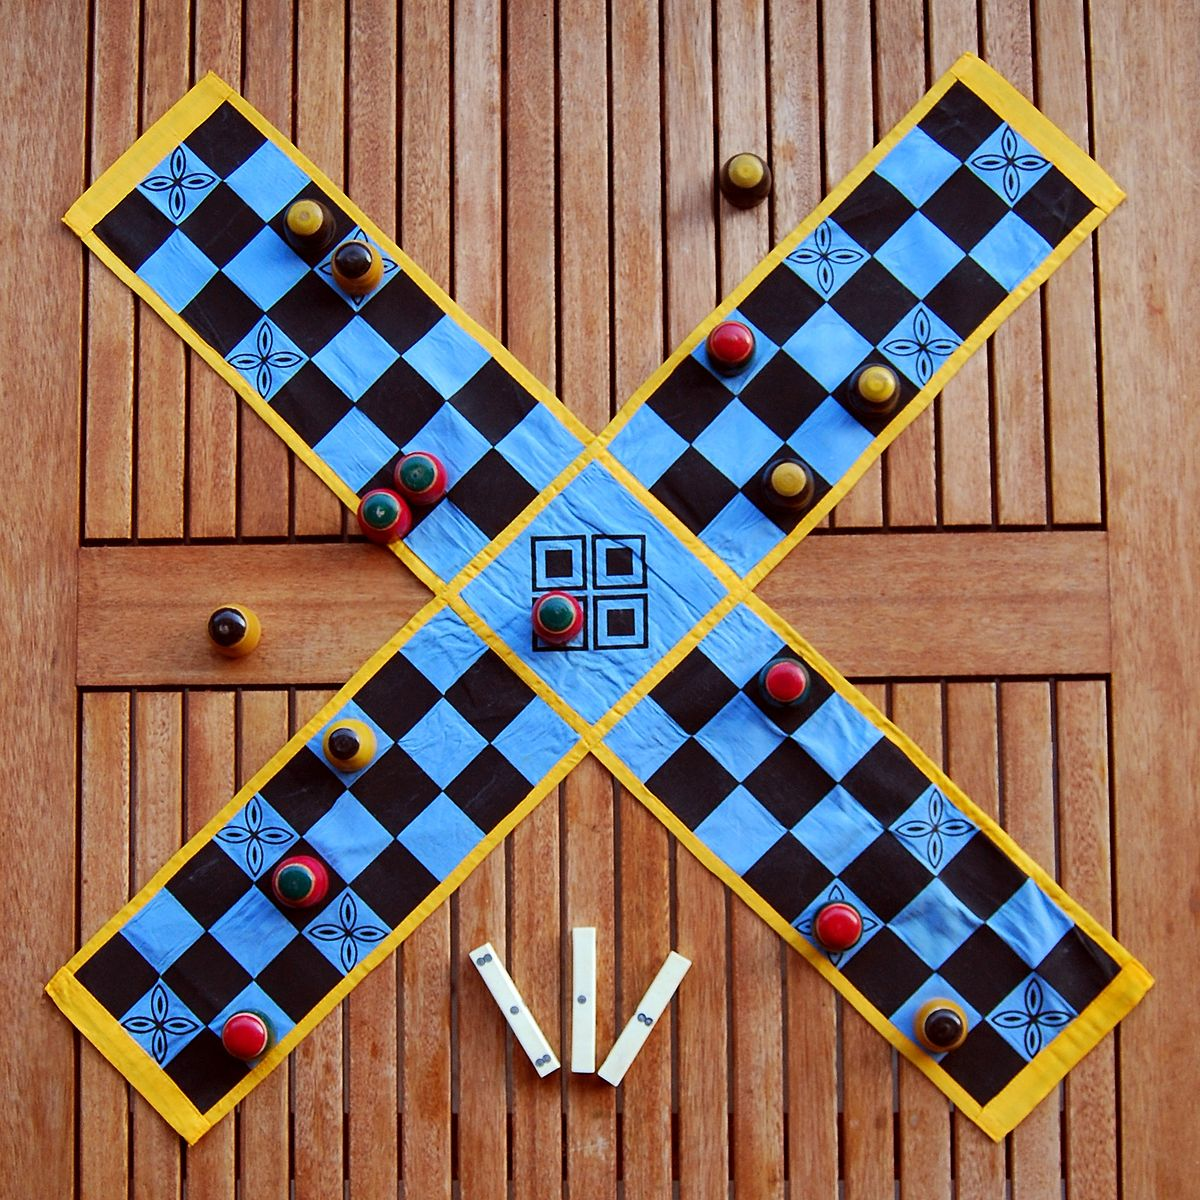
\includegraphics[width=0.4\textwidth]{images/pachisi.jpg}}
    \caption{Pachisi}
\end{figure}
Mittlerweile existieren auch viele Abk\"ommlinge und Varianten mit ver\"anderten Regeln oder Spielfeldern. Allen Varianten ist jedoch gemein, da\ss sie ein symmetrisches Spielfeld besitzen und analog entwickelt wurden. Man kann vermuten, dass mit asymmetrischen Spielfeldern experimentiert, dies jedoch
nicht weiter verfolgt wurde, da es ungleich schwieriger ist, eine asymmetrische Konfiguration zu finden bei der die Chancengleichheit und somit der ausgewogene
Spielspass f\"ur alle Spieler gegeben ist. Dennoch ist der Reiz dieses Szenarios nicht zu verachten, da die Freiheit bei der Gestaltung asymmetrische Spielfelder
\"au\ss erst fruchtbar f\"ur die Entwicklung interessanter Spielvarianten, welche sich nicht in das relativ starre klassische Korsett einpassen m\"ussen, ist. Die gr\"o\ss te
H\"urde in diesem Bereich ist also die m\"uhelose Erstellung eines experimentellen Spielfeldes, um dieses unmittelbar auf seine Spielspa\ss eigenschaften zu testen.

Zu diesem Zweck wurde eine Java-Applikation entwickelt, welche einen Spielfeldgenerator implementiert, der mittels einer DSL variable Spielfelder erzeugen kann. Im Verlauf der Architekturdokumentation wird sowohl auf die Besonderheiten der Implementierung, als auch auf die verwendeten Design-Patterns und den Code-Generierungsansatz eingegangen. Abschlie\ss end wird ein Fazit formuliert, das die Erfahrungen und Ergebnisse zusammenfasst.


\section{Anforderungen an die Applikation}

Grundlegend an die Anforderungen ist die Tatsache, dass das Programm f\"ur Programmierer und Designer gleicherma\ss en benutzbar sein mu\ss. W\"ahrend der Designer sich vollst\"andig auf die Entwicklung interessanter Spielfelder konzentrieren k\"onnen mu\ss, d.h. man kann keine Programmierkenntnisse vom ihm verlangen, darf dies den Programmierer nicht daran hindern, die Applikation weiter zu entwickeln, also
in den Bereichen grafisches Erscheinungsbild, Regeln, K\"unstliche Intelligenz und Spielfeld Ver\"anderungen vorzunehmen. Aus diesen Gedanken
heraus haben sich die grundlegenden Anforderungen gebildet.
Die Applikation sollte m\"oglichst unabh\"angig vom Betriebssystem lauff\"ahig sein. Da eine starke Eigenschaft von Java die Portabilit\"at und
Lauff\"ahigkeit auf vielen unterschiedlichen Ger\"aten ist, wurde diese als Entwicklungsprogrammiersprache gew\"ahlt. Dadurch lassen sich auch Abk\"ommlinge
des Prototypen (exemplarisch MobileApp) gut planen und umsetzen. Die verbindende Technologie zwischen Programmierer und Designer ist das ausgereifte
Codegenerierungs-Tool Antlr, welches das $.csv$-Dateiformat von Haus aus beherrscht und f\"ur die programmierkenntnislose Erstellung von Spielfeldern
geeignet ist. Diese Aufstellung des Technologiestacks erlaubt einen wechselseitigen Workflow ohne gro\ss e Unterbrechungen. Der Designer kann
mit der aktuellen Version neue Spielfelder erzeugen oder bereits designte testen und Vorschl\"age zum Regelwerk machen. Der Programmierer
kann solche Feature-Requests umsetzen und einspielen, woraushin der Designer wieder iterieren kann. Beide kommunizieren also vorrangig
\"uber die Grammatik des Spiels und sind nicht prim\"ar an technische Beschr\"ankungen gebunden. Weiter kann der Programmierer kann unabh\"angig vom Designer
an der graphischen Erscheinung der View und dem Verhalten der k\"unstlichen Spieler arbeiten. F\"ur den Designer ist eine einfache Bedienung
wichtig, d.h. es wird nur von ihm verlangt mit der View zu kommunizieren und neue Spielfelder zu erzeugen, aber keine weiteren Deploy-Prozesse zu beachten.


- os unabh\"angig lauff\"ahig
- trotz development dauerhaft lauff\"ahiger zustand (f\"ur designer)
- keine programmierkenntnisse, um neue spielfelder zu erzeugen und zu testen
- erweiterbarkeit der regeln
- erweiterbarkeit f\"ur k\"unstliche spieler
- einfachste bedienung (nur maus + linke maustaste)

  usage f\"ur designer: entwickele spielfeld, starte generator, starte applikation,
    vorschl\"age an den programmierer zur weiterentwicklung
  usage f\"ur programmierer:
    entwickele view 
    erweitere regeln (controller: businesslogic, model: neue datenfelder)
    erweitere generator/grammatik
    nach implementierung designer neue version zur verf\"ugung stellen



\section{Genutzte Design Pattern}
\subsection{MVC}
  F\"ur die Abbildung eines Brettspiels in digitaler Form bietet sich das klassische Model-View-Controller Pattern an.

  Dabei ist zu beachten, das die Dreieckbeziehung im MVC nicht symmetrisch, sondern hierarchisch implementiert wird, da sonst die Verantwortlichkeiten
  von Model, View und Controller aufgeweicht werden und feste Kopplungen sowie Spaghetti-Code beg\"unstigt werden. Konkret bedeutet das, das der Controller das Model und die View kennt, die View jedoch nur, um seine Callbacks auf asynchrone Events (z.B. Benutzereingaben) der View anzumelden. Als Controller darf er im Zuge des Spielablaufs im Model Ver\"anderungen vornehmen. Die View kennt das Model, darf aber nur daraus lesen, um sich selbst, d.h. die grafische Darstellung der Applikation auf dem aktuellsten Stand zu halten. Das Model als Datenhalter kennt niemanden, stellt aber Lese- und Schreibfunktionen zur Verf\"ugung. Diese Aufteilung ist noch weiter ausbauf\"ahig, bei zunehmender Komplexit\"at w\"are es sinnvoll f\"ur die
  Einhaltung der Verantwortlichkeiten EventDispatcher-Pattern hinzuzuf\"ugen. Dadurch k\"onnen das Model und die View Events bei Eingabeereignissen oder Datenver\"anderungen senden, ohne dass die lose Kopplung verlorengeht. Im Prototypen wurde sich dagegen entschieden, da ein einzelner Aufruf f\"ur die GUI-Aktualisierung pro Spielzug und die Anmeldung zweier Callbacks den Mehraufwand nicht rechtfertigten.

\subsection{Singleton}

Die Applikation soll stets ein lauff\"ahiges Mensch-\"arger-dich-nicht-Spiel repr\"asentieren, welche aufgrund des Designeraspekts ohne komplizierte Laufzeiteinstellungen auskommen oder Kommandozeilenparametern zu starten sein mu\ss. Es ist also nicht erw\"unscht, das mehrere Instanzen der Hauptklassen erzeugbar sind, da dies zu kompliziertem Initialisierungscode mit entsprechend notwendigen Konfigurationen von au\ss en in den Toplevelschichten f\"uhren w\"urde. Im Code wird dies dadurch reflektiert, dass die Hauptklassen von Model, View und Controller als Singletons implementiert sind.
Die Eleganz dieser Variante zeigt sich in der \"ubersichtlichen \texttt{Main}-Klasse, in der nur noch die Singletons instanziiert und miteinander verkn\"upft werden. S\"amtliche Weiterentwicklung des Programms kann innerhalb der MVC-Komponenten erfolgen, ohne das die \texttt{Main} angepasst werden mu\ss .

\section{Implementierung}
Die Applikation wurde in einem 2er-Team entwickelt. Als erstes wurde die Grammatik definiert, damit dann parallel
ein Grundger\"ust der Applikation $MenschAergerDichNicht$ entworfen und der Generator $MADPlayfieldGenerator$ geschrieben werden konnte. Nachdem beide Projekte minimal lauff\"ahig waren, haben sich die Entwicklungsrollen iterativ vermischt, bis der Prototyp ausreichend angereichert und getestet
war.

F\"ur die einfache und konfigurationslose Verkn\"ufpung der beiden Projekte wurde ein relativer Pfad, welcher lediglich verlangt, dass sich beide Projekte nebeneinander in einem Ordner befinden und ein fester Name $GEN\_PlayfieldCreator.java$ f\"ur die erzeugte Quellcodedatei gew\"ahlt. Dadurch konnte die Code-Generierung mit einem einzigen Befehl�permanent angewendet werden.

\subsection{Grammatik/DSL}
  Die Grammatik des Spiels enth\"alt Symbole f\"ur alle m\"oglichen Spielfeldtypen und deren Verkn\"upfungen zum Nachfolgefeld.
  Es k\"onnen Spielfelder f\"ur 2 bis 4 Spieler definiert werden. Das reichte f\"ur den Prototyp aus und kann ohne besondere
  Schwierigkeiten erweitert werden.
  Die Spielfeldtypen eines klassischen Mensch-\"arger-dich-nicht-Spiels sind wie folgt im Code und in der DSL realisiert:

\begin{table}[h!]
  \centering
  \caption{Tiletypes}
  \label{tab:table1}
  \begin{tabular}{ccc}
    \toprule
    Java & DSL\\
    \midrule
    HOME & H[p]\\
    START & S[p]\\
    GOAL & G[pn] \\
    WAY & W[n] \\
    TOGOAL & W[n]G[n] \\
    NONE & NO \\
    \bottomrule
  \end{tabular}
\end{table}

Das K\"urzel $n$ steht f\"ur die Knoteninformation, welches Feld dem betreffenden folgt, dies kann eine der 4 Himmelrichtungen $N$,$S$,$W$,$E$ sein. Das andere K\"urzel $p$ hingegen enth\"alt die Spielernummer 1-4. Einen kleinen Spezialfall stellt der Typ $TOGOAL$ dar, das dies ein Spielfeldtyp ist, welcher zwei Nachfolgeknoten enth\"alt. Der zweite ist die Abzweigung in die Zielfelder des jeweils passenden Spielers. Durch die knotenbasierte Definition
der Spielfelder ist dies jedoch problemslos implementierbar (siehe \ref{code}) und auch erweiterbar.
Da das $.csv$-Format zeilenbasiert ist, wurde f\"ur den Prototypen entschieden, nur matrixartige Spielfelddefinitionen zuzulassen. Dies wird im unten erkl\"arten \texttt{PlayFieldMetaListener} \"uberpr\"uft.

\subsection{Generator}

Um aus den $.csv$-Dateien eine $.java$-Datei zu erzeugen, musste ein zweistufiger Parser geschrieben werden. Der erste Parser \texttt{PlayFieldMetaListener} ermittelt Metadaten des Spielfeldes, die der zweite Parser \texttt{PlayFieldSemanticListener} ben\"otigt, um den spielfelderzeugenden Code generieren zu k\"onnen. Dazu wird die $.csv$-Datei einmal durchlaufen um die Metadaten zu akkumulieren. Zu diesen geh�ren die Anzahl der Spieler, die gleichzahligen Home- und Endpositionen der jeweiligen Spieler, das Vorhandensein genau eines Startfeldes pro Spieler sowie die Anzahl der Zeilen und Spalten der $.csv$-Definition. Etwaige Fehler werden mit einer Abbruchsmeldung quittiert. Sind alle Metadaten gesammelt, was erst nach einem vollst�ndigem Scan garantiert ist, kann der \texttt{PlayFieldSemanticListener} gestartet werden, da dieser die Metainformationen ben�tigt, um den Code f�r die Spielfeldverkn�pfungen mit den nun bekannten Indizes zu generieren.
Die generierte Datei enth�lt danach die Zugriffsfunktionen 

\texttt{getNumRows},
\texttt{getNumColumns},
\texttt{getNumPlayers} und
\texttt{getNumPiecesPerPlayer}
f�r die Metadaten und die spielfelderzeugende Funktion \texttt{createPlayfield}, welche wie in \ref{abschnitt playfieldklasse} benutzt werden. Wie man an einer beispielhaften Zeile \texttt{playfield.getTile(0, 6)// 
.setType(TileType.START)//.setNext(playfield.getTile(1, 6))//.setPlayerID(2);} innerhalb dieser Methode sehen kann, werden die matrixartige Struktur der $.csv$-Datei und die gewonnenen Metadaten verwendet, um die Knotenverkn�pfungen zwischen den einzelnen Spielfeldern zu erstellen. Nach dieser Zuordnung kann auf die Koordinatenwerte der Felder vollst�ndig
verzichtet werden.

meta parser:
 liest spielfelddatei und ermittelt metadaten, also daten das ganze spielfeld betreffend und positionsunabh\"angig
 - spieleranzahl
 - ein startfeld pro spieler
 - gleiche anzahl an home und goal feldern pro spieler
 - h\"ohe, breite der spielfeldmatrix
 - daten werden als getter im genierten code bereitgestellt

semantic parser
 - liest die einzelnen felder
 - verkn\"upft die knoten
 - generiert den erzeugungscode des spielfeldes

Die so generierte Datei enth\"alt die Methoden \texttt{getNumRows}, \texttt{getNumColumns}, \texttt{getNumPlayers} und \texttt{getNumPiecesPerPlayer} mit den ermittelten Daten des Meta-Parsers
sowie die Methode \texttt{createPlayfield} des Semantic-Parsers, welcher eine zu bef\"ullende \texttt{Playfield} Instanz �bergeben wird.



  \subsection{Applikation}

  Im folgenden werden die einzelnen Klassen der Applikation vorgestellt.

\subsubsection{Game}

Die Klasse \texttt{Game} ist das Herz der Applikation. Als Hauptcontroller h\"alt er Referenzen zum Subcontroller \texttt{PlayerController}, zur View \texttt{GUI} zum Model \texttt{Playfield}. In der \texttt{Main}-Methode wird die Applikation \"uber \texttt{ Game game = Game.getInstance(); game.init(playerController, playfield, gui);} zusammengesetzt. Im \texttt{Game}-Controller finden sich Methoden zur Eingabebehandlung: mit \texttt{onStartButtonClicked} kann ein neues Spiel begonnen werden. Mit \texttt{onRollDiceButtonClicked} wird W\"urfeln der menschlichen Spieler verarbeitet und mit \texttt{onMouseClicked} werden Klicks auf das Spielfeld verarbeitet. Dabei handelt es sich um Spielfigurbewegungen der menschlichen Spieler.
Zum Steuern des Spielablaufs existieren die Methoden \texttt{startGame}, mit der ein neues Spiel initialisiert wird.
\texttt{checkForWin} pr\"uft nach jedem Spielzug, ob ein Sieger feststeht und beendet gegebenenfalls das Spiel durch
\texttt{endGame}.
\texttt{turn} leitet einen Spielzug ein. Im Falle eines menschlichen Spielers wird anschlie\ss end auf Eingaben gewartet, bei einem k\"unstlichen Spieler wird das W\"urfeln automatisch ausgef\"uhrt und die KI \"uber \texttt{turnKI} zur Spielfigurenbewegung angesteuert. Die zufallsgenerierten W\"urfelwerte
werden von \texttt{rollDice} zur\"uckgegeben. F\"ur die Logik innerhalb des Spielablaufs existieren die Methoden
\texttt{prepareBonusRoll}, welche gesondert nach einer gew\"urfelten 6 angesteuert wird und im Falle einer anderen gew\"urfelten Zahl
\texttt{prepareNextPlayer}, wenn der entsprechende Spieler seinen Zug abgeschlossen hat.

Die zentrale Methode \texttt{tryMove} wird angesteuert, wenn eine Spielfigur von einem -gleichg\"ultig ob menschlich oder k\"unstlich- Spieler bewegt werden soll. In ihr werden die Regeln zur validen Bewegung der Spielfigur \"uberpr\"uft, der Zug wenn m\"oglich ausgef\"uhrt (wodurch sich das Model \"andert) und die Validit\"at als \texttt{boolean} Wert zur\"uckgegeben. Durch den R\"uckgabewert wird gesteuert, ob im Falle einer KI eine andere Spielfigur bewegt oder wieder auf Mauseingaben des Benutzer gewartet werden soll. War der Zug valide, wird zum n\"achsten Spieler im Spielverlauf weitergegangen. Unterfunktionen von \texttt{tryMove} sind \texttt{cantMoveOut}, welche die Zwangsregel, dass man eine Spielfigur -wenn m\"oglich- heraussetzen muss und
\texttt{isValidTarget}, welche \"uberpr\"uft, ob das Zielfeld einer Spielfigur ein valide Position darstellt. Auf die letztgenannte Methode soll kurz genauer eingegangen werden, da sich in ihr die Vorteile des knotenbasierten Spielfeldes zeigen. Zum Ermitteln eines legales Spielzugs der Spielfigur wird zuerst das Feld, auf dem die Spielfigur sich befindet, referenziert und nachfolgende die Methode \texttt{getTargetTile} auf dem referenzierten Spielfeld aufgerufen, dessen Implementierung in Abbildung \ref{ code} zu sehen ist. Mithilfe der Nachfolgeknoteninformation wird solange der n\"achste Knoten referenziert, bis entweder kein Nachfolgeknoten existiert (im Falle des letzten Zielfeldes eines Spielers) oder die gew\"urfelte Schrittweite erreicht ist.
Zu beachten ist, da\ss keinerlei planaren Positionsinformationen ben\"otigt werden. Dadurch ist es m\"oglich, Wege durch v\"ollig frei gestaltete Spielfelder
zu suchen. Weiterhin lassen sich zwanglos neue Spielfeldtypen f\"ur exotischere Spielvarianten hinzuf\"ugen.

\subsubsection{PlayerController}
     
Der \texttt{PlayerController} dient lediglich der Verwaltung der Spieler. Durch diese zus\"atzliche Kapselung wird jedoch der \texttt{Game}-Controller
nicht unn\"otig mit spielablauffremden Methoden aufgebl\"aht, wenn die Spielerverwaltung durch erweiterte Spielmodi komplizierter wird. Dazu geh\"ort beispielsweise die Anmeldung der Spieler (menschlich oder k\"unstlich) beim Spielstart und die sp\"atere Abmeldung f\"ur Spielmodi mit mehreren Siegerpl\"atzen.

  View: 
    GUI
       -verantwortlich f\"ur den Rahmen, fenstergr\"o\ss e usw
    PlayfieldPanel
        - rendering des spielfeldes (tiles, pieces)

  Model:
    Playfield
      - alle tiles
    Tile 
      - knoteninformationen
      - referenzinformation \"uber pieces
    Player
      - enth\"alt seine pieces
      Ableitungen: KIPlayer/HumanPlayer



  implementierungsvorteile durch knotenbasierte spielfeldelemente


    -erzeugt eleganten regel code durch tiletypen und lookahead function
    -einfache erweiterung neuer tiletypen und regeln
    -nat\"urlich abbildung der regeln in code


    Typendefinitionen: tileType

    beispiele zeigen:
    if (tile.TILETYPE == START \&\& tile.hasPiece())) // cant move to start, its not free


\section{Fazit}

knoten ansatz sehr gut geeignet f\"ur erweiterung/generalisierung der spielfeldgenerierung
einsatz passender pattern an den richtigen stellen f\"ur weiterentwicklung der software
(ki subclass, spielregeln)

grammatik zeilen/spalten gebunden (keine planar frei plazierbare tiles ohne x, y beschr\"ankung)
aber m\"oglich, tiles nur knotengebunden, dh
zus\"atzlicher editor f\"ur graphisches design von csv-vorlagen m\"oglich
verschieben von graphischen elementen hat keinen einflu\ss  auf knotenverkn\"upfungen

% conference papers do not normally have an appendix


% use section* for acknowledgment
\section*{Acknowledgment}


The authors would like to thank...


\begin{thebibliography}{1}

\bibitem{IEEEhowto:kopka}
H.~Kopka and P.~W. Daly, \emph{A Guide to \LaTeX}, 3rd~ed.\hskip 1em plus
  0.5em minus 0.4em\relax Harlow, England: Addison-Wesley, 1999.

\end{thebibliography}




% that's all folks
\end{document}


